\chapter{Evaluation}
\label{chap:evaluation}

The online interactive map was evaluated in two different studies. Beforehand, it was published online and merged to the existing energy chart website to make it available for a large audience. In addition, an online survey was prepared to evaluate the map and deployed online to assess the impact, usefulness, and usability of the of this visualization tool.  This online study evaluates the map on two different characteristics. The first study was focusing on the representational aspects of the map and the second was aiming at the usability of the map and its interactive functionality. The goal of this survey was to accumulate qualitative feedback on the map interface, visualization techniques, usability, and scopes of accessing data. In this chapter, the survey studies and their results are analyzed, explained, and discussed in detail.

\section{Online Survey Setup}
\label{chap:suveySetup}

An online survey application is used to create and host the survey. LimeSurvey \footnote{Official LimeSurvey Website, \url{https://www.limesurvey.org/} (last accessed on \today)} is a free and open source tool for publishing on-line surveys. It provides wide variety of features for creating graphical analysis of survey results. Four different question groups with a brief introduction about the purpose of this evaluation and a little usage guide of the visualization tool were created using this survey application. Therefore, users can explore the map and discover the functionality before participating in the survey. The participants were invited over the email and social media. They did not get any reward for participating in the online survey. None of the survey questions were mandatory, therefore participants were not required to answer every question. 

In the short introduction, all the participants were informed about the purpose of making this visualization tool followed by a short description about the usability, and some tasks they need to perform for using the map and extracted the data out of it. The tasks were divided into the following steps:

\textbf{Exploring power plant information:}\\
In the description, participants were asked to click on the map marker to view the information of each power plants from the pop-up box. 

\textbf{Use navigation menu for interaction:}\\
In the description, participants were told to use the navigation menu for selecting each source category and for rendering the power lines on the map.

\textbf{View hourly production data:}\\
In the description, participants were told to use the “Go to Energy Charts” link to view the hourly production data on the energy charts.

\textbf{Compare power plants production:}\\
In the description, participants were told to use the "Compare" button to  compare between power plants in a comparison table.

\textbf{View hourly production data of multiple power plants:}\\
In the description, participants were told about the “Compare on Energy Charts” link that appears under the comparison table. By clicking on the link, they can see the hourly production data of the power plants, which are in the comparison list, on the Energy Charts. 

After the short introduction, there were four different question groups to empirically evaluate the interface and usability of the map. In total, there were 20 questions in the online survey and participation time was estimated about 5 minutes.  

\subsection{Question Groups}
\label{sssec:quesGroup} 

\subsection*{Introduction}
\label{sssec:intro}

The first question group was about the demographic information. Participants were asked to mention their gender, age, and professional area of working, besides that their frequency of using interactive maps and their acquaintance with the German power plants and its electricity production were asked. 

\subsection*{User Interface Evaluation}
\label{sssec:uiEval}

In this group, participants were asked to evaluate the user interface and its components especially about the cluster view, map markers, power lines, and comparison table. A collection of the demographic question, rating scale, and multiple choice question were asked for this evaluation. 

\subsection*{Map Usability Test}
\label{sssec:MUtest}

In this group, participants were asked to evaluate the usability and usefulness of this visualization tool. Participants were also requested to leave some comments only if it was difficult to use. 

\subsection*{Comments or Suggestion}
\label{sssec:cORS}

Participants were asked to comment on this complete work package and its features as well as requested to provide suggestions on adding new features or ideas.  

\section{Survey Results and Discussion}

In this section, the result of survey questionnaire of each question group and the qualitative comments and consequences derived from these visions are discussed. 

\subsection{Summary of Participants and Their Backgrounds}

The goal of this question group was to get an idea about the participants, their professional background, age ratio, and their familiarity with German power plants. In addition, we asked how frequently they use interactive maps in their daily life. For our online research study, 23 participants (19 males, 2 females, 2 did not answer), from different levels of expertise, participated in the survey. Participants belong to different age groups where 50\% with an average age of 27 years, 35\% are with an average of 53 years and 15\% are with an average age of 36 years (see Figure \ref{fig:participantBack}). In total, 19 full and 4 partial survey reports were submitted. 

\begin{figure}
  \begin{center}
\subfloat[Age ratio of participants\label{fig:age}]
  {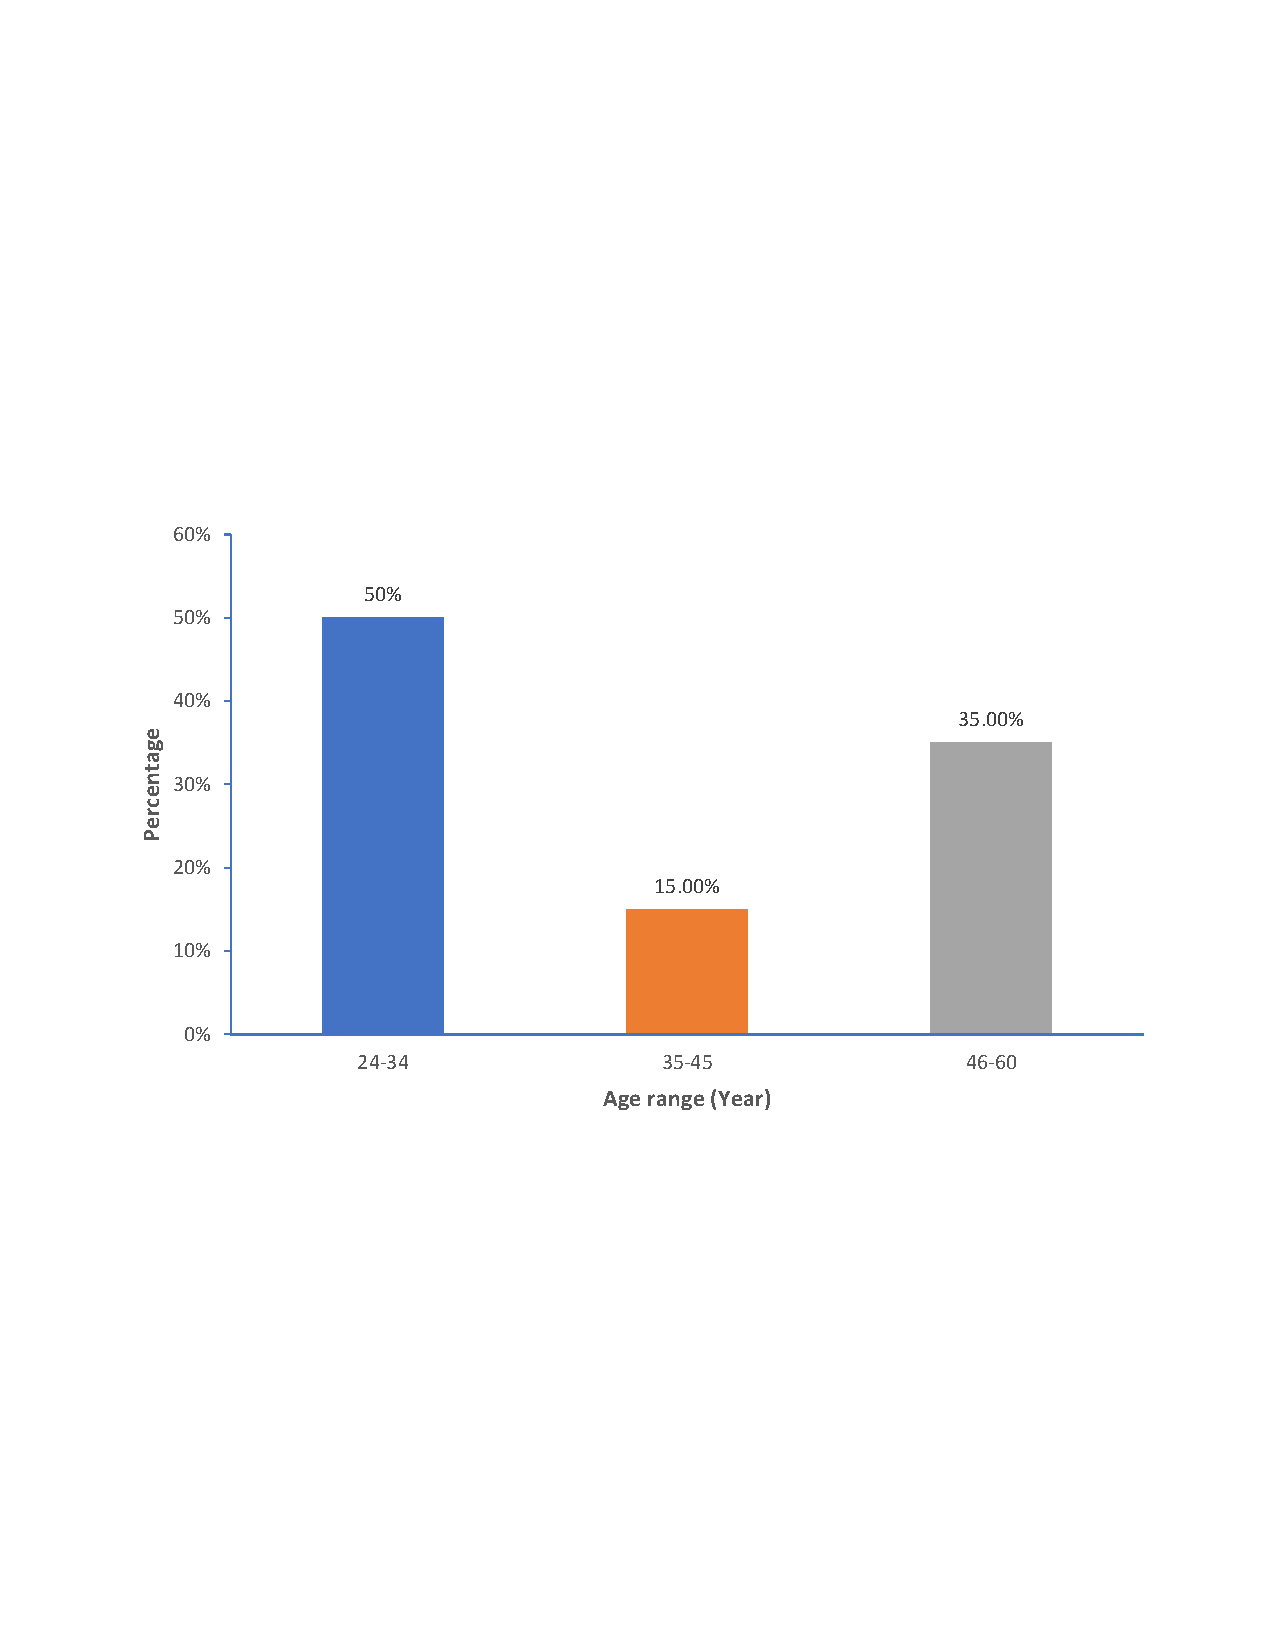
\includegraphics[width=.45\linewidth]{study/age}}\hfill
\subfloat[Professional backgroud of survey participants\label{fig:ageJob}]
  {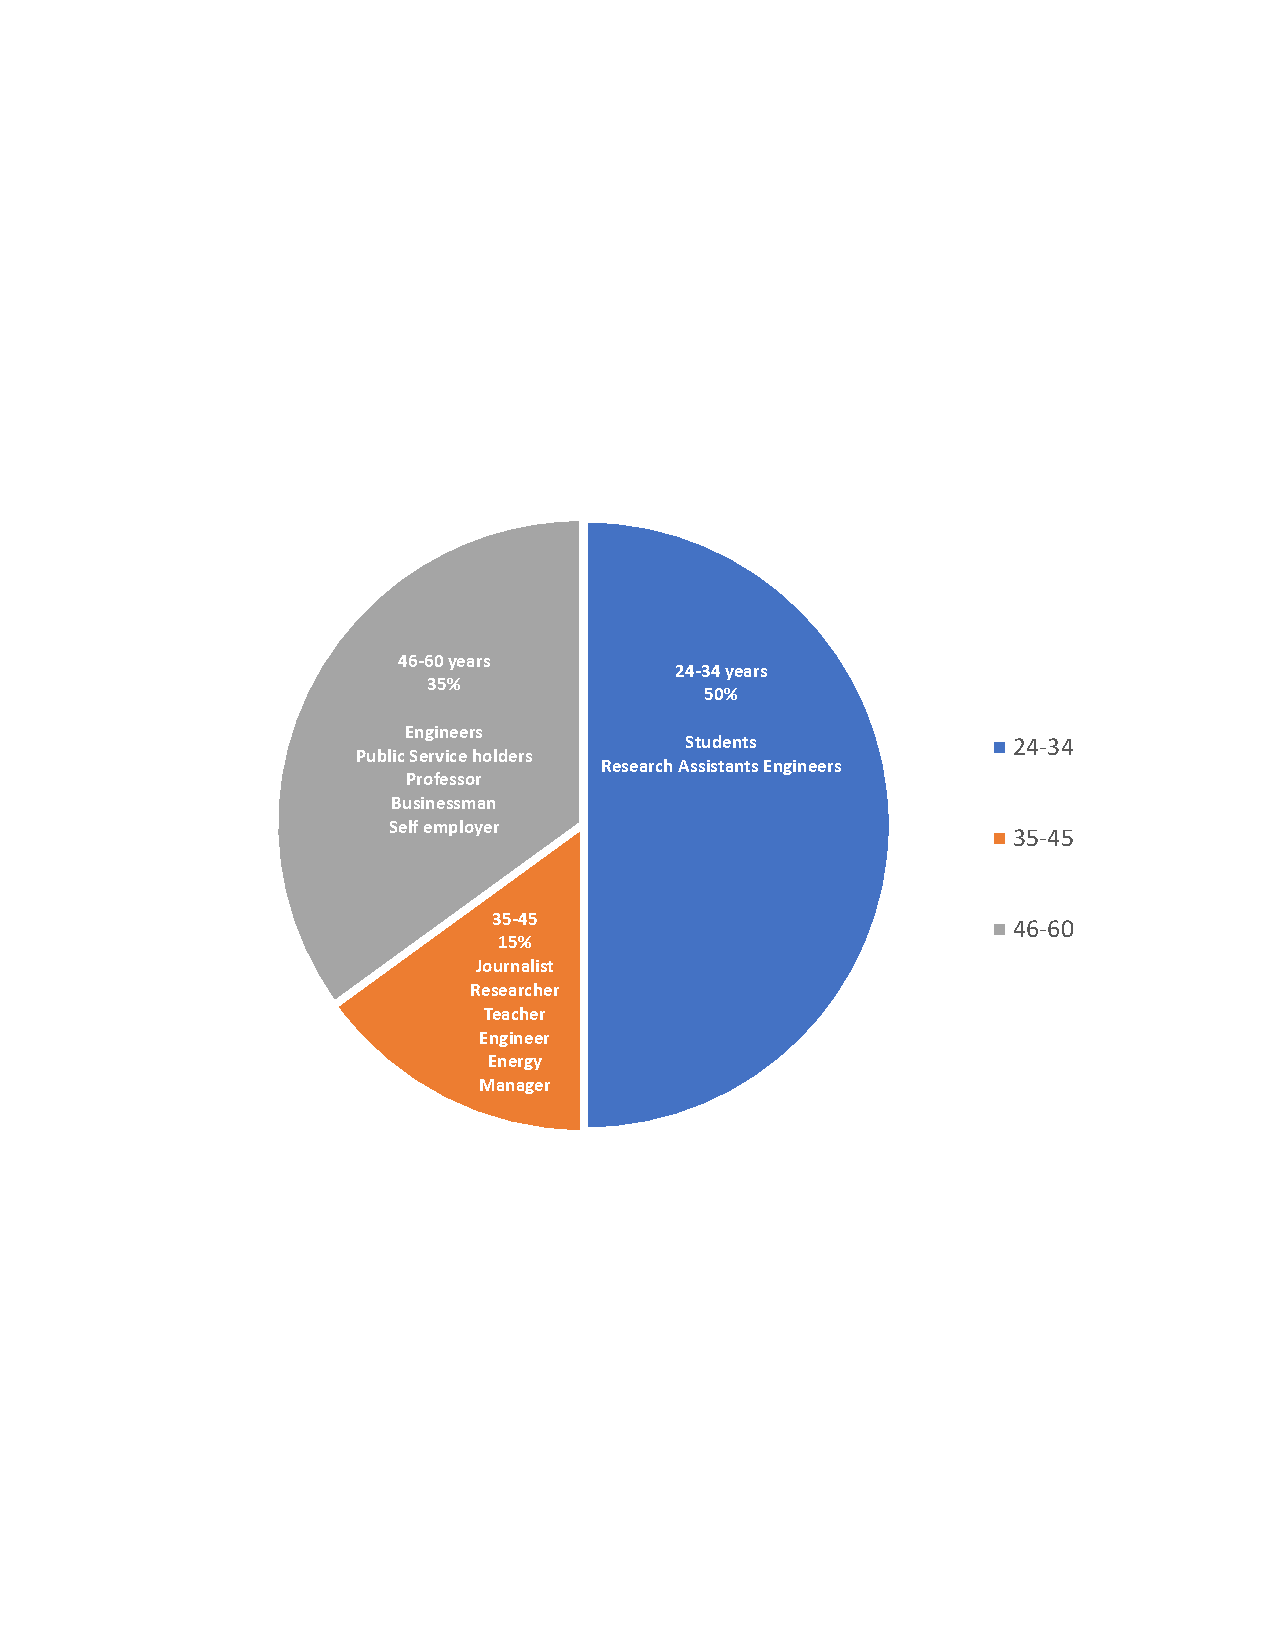
\includegraphics[width=.45\linewidth]{study/pie}}
\hfill
\caption{Age ration and professional background of survey participants}
\label{fig:participantBack}
\end{center}
\end{figure}

Summary of this question groups tells us that almost 50\% of the participants who are comparatively younger than other participants are familiar with German power plants and their production to some extent.  Whereas other participants, who belong to older age groups, are somewhat or very much familiar with it (see Figure \ref{fig:familiar}). After digging up the data more deeply it has been noticed that younger participants are mostly students, research assistants, and engineers. However participants older than other group are professors, businessman, and working in the energy industry (see Figure \ref{fig:ageJob}). Nevertheless, the participants having no idea about German power plants also exists in all age groups. On the other hands, concerning the frequency of using interactive map per week, a maximum number of participants (around 70\%, see Figure \ref{fig:mapUsage}) use interactive map at least once or twice in a week. Therefore, we assumed that user would find the tool and its functionality easy to use.

\begin{figure}
  \begin{center}
    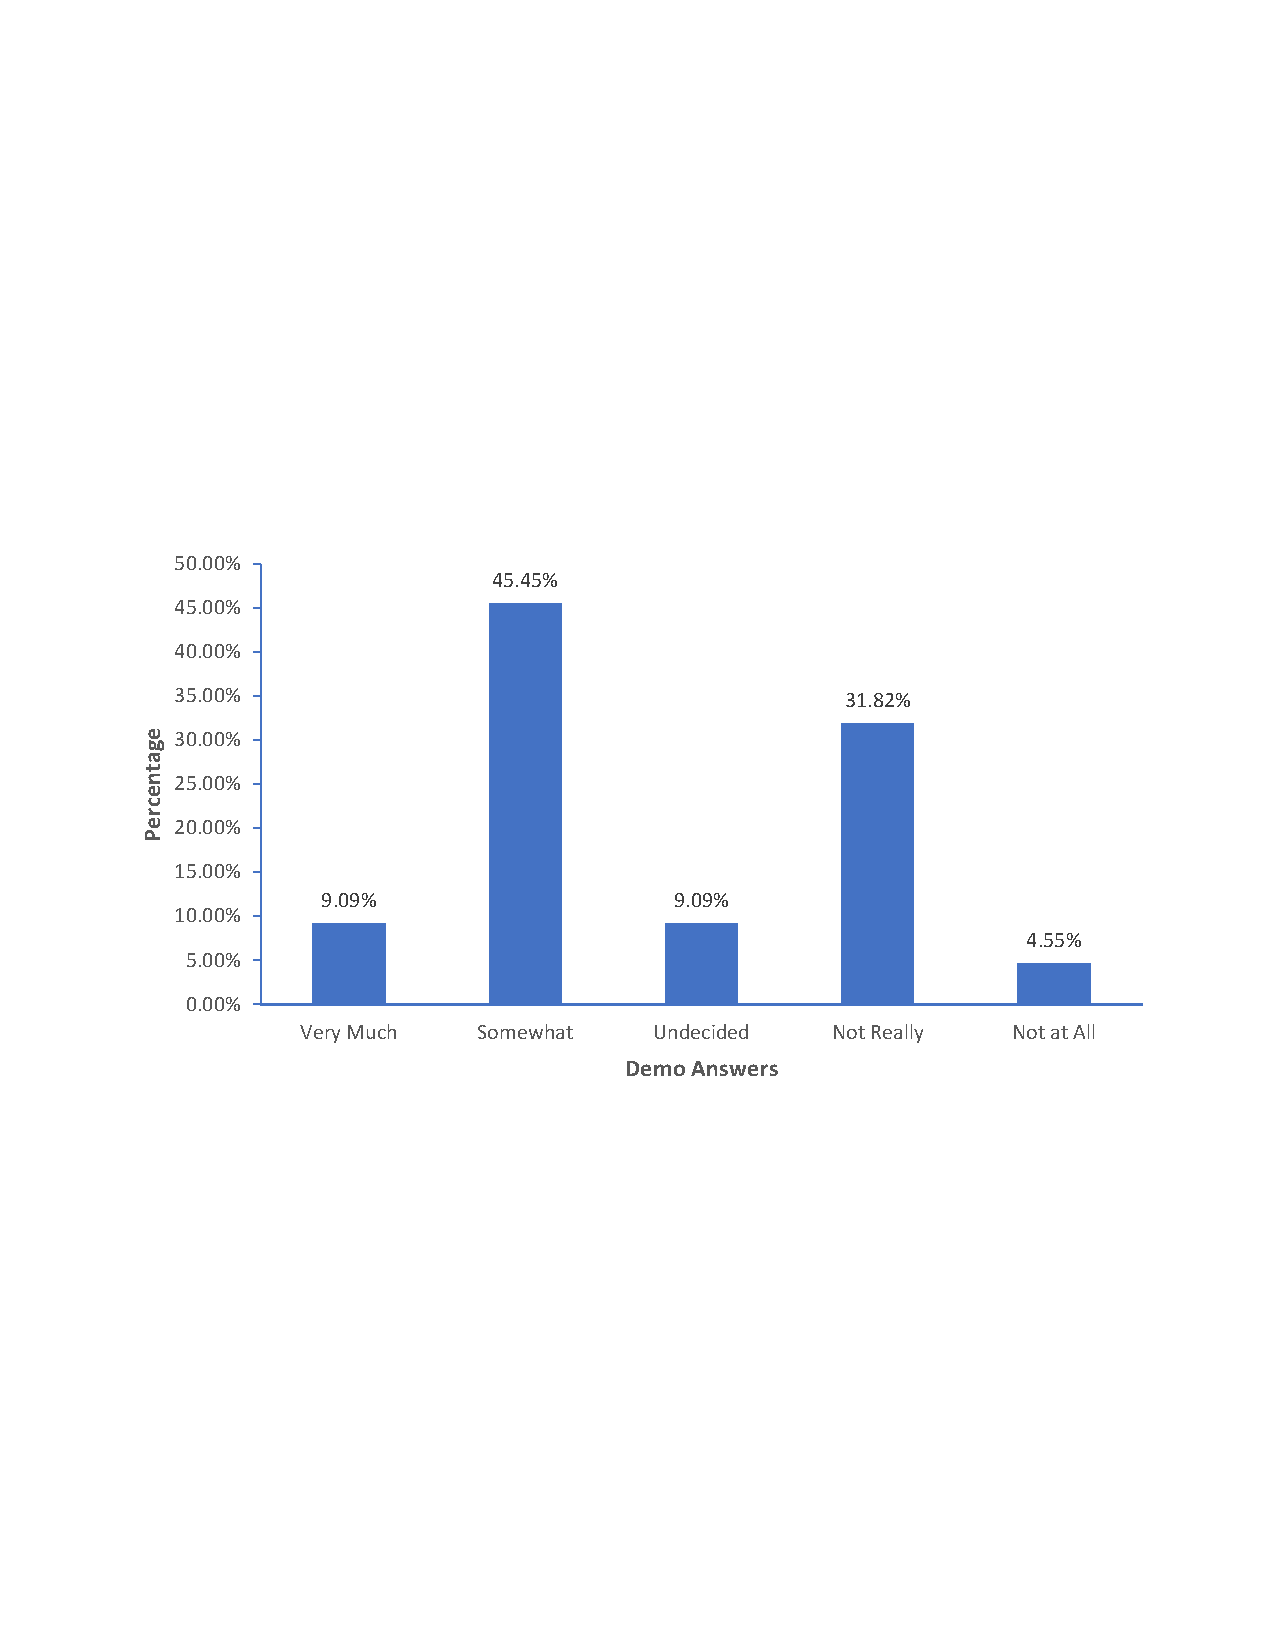
\includegraphics[width=1\textwidth]{study/familiar}
    \caption{Familiarity with German power plants and their production}
    \label{fig:familiar}
  \end{center}
\end{figure}

\begin{figure} 
  \begin{center}
    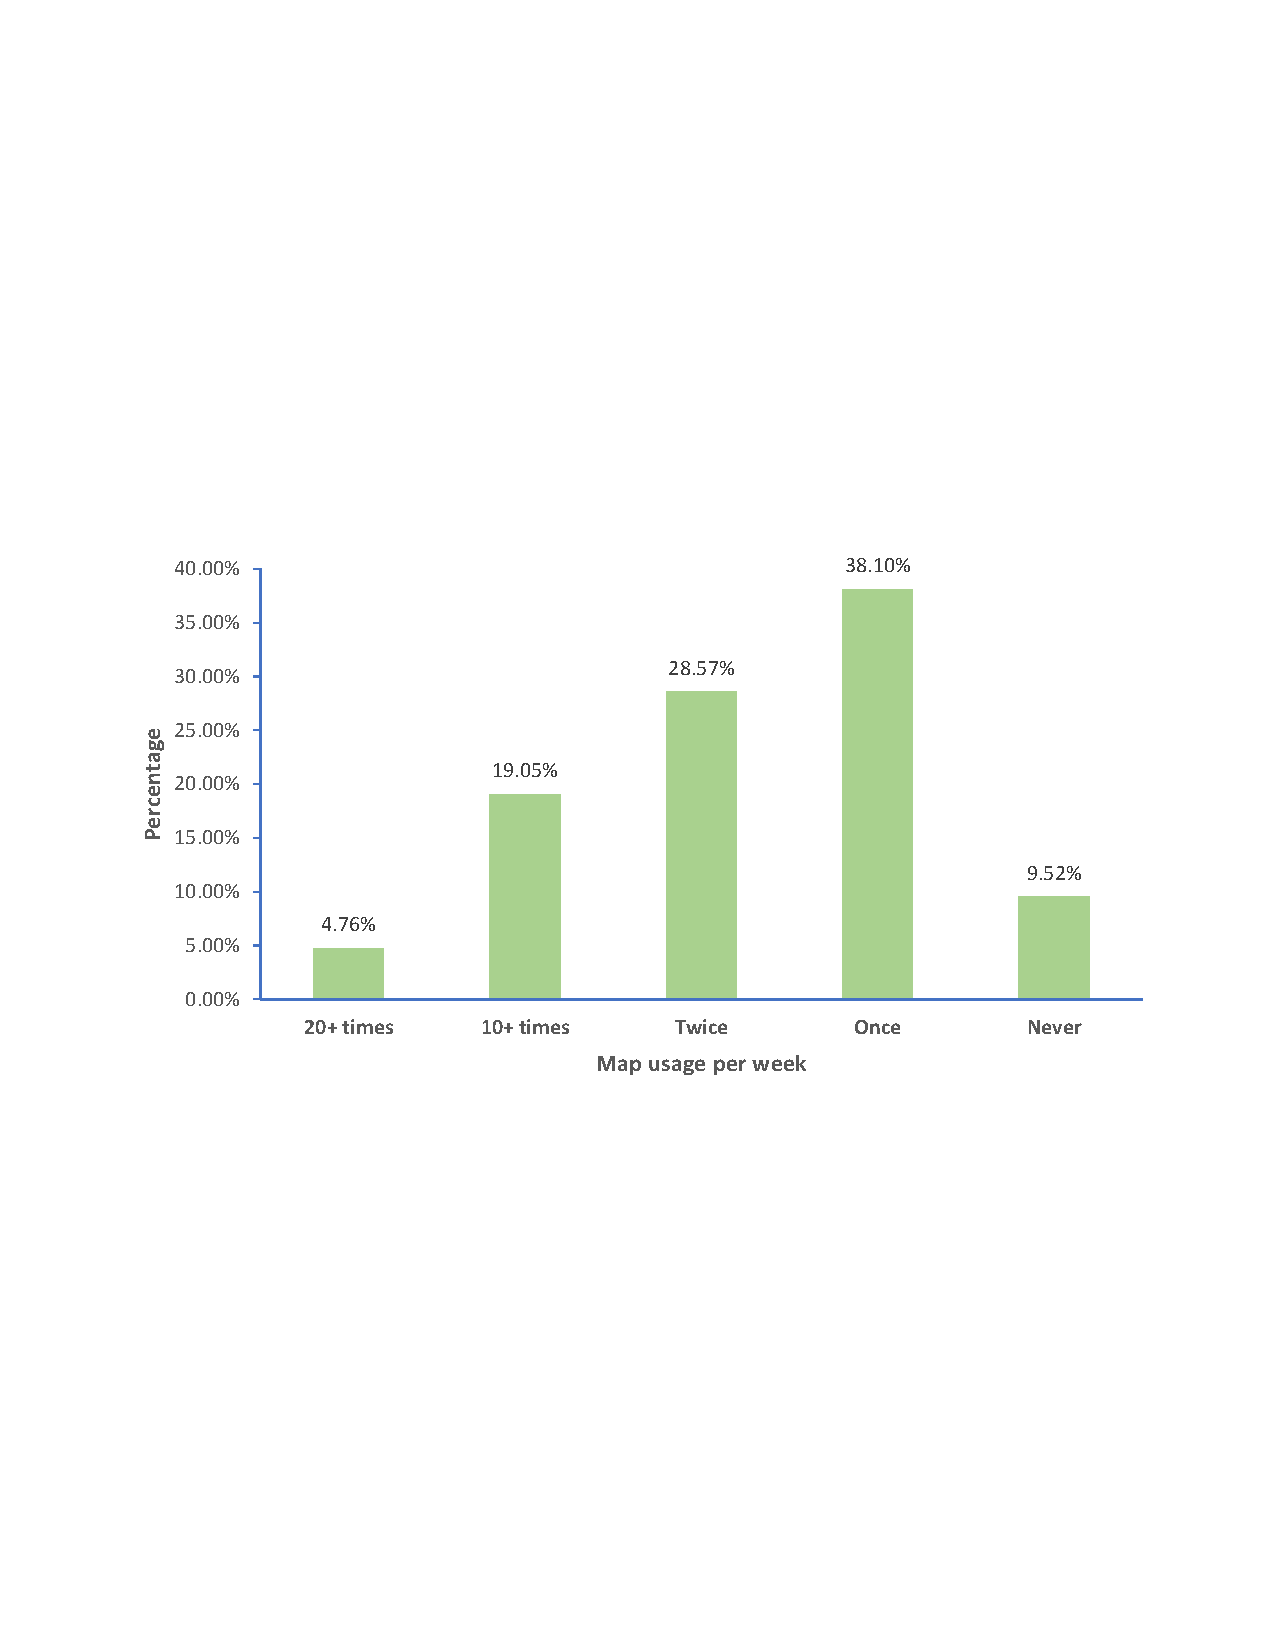
\includegraphics[width=1\textwidth]{study/frequency}
    \caption[participants frequency of using interactive map per week]{The result of online survey - participants frequency of using interactive map per week}
    \label{fig:mapUsage}
  \end{center}
\end{figure}

\begin{figure}
  \begin{center}
    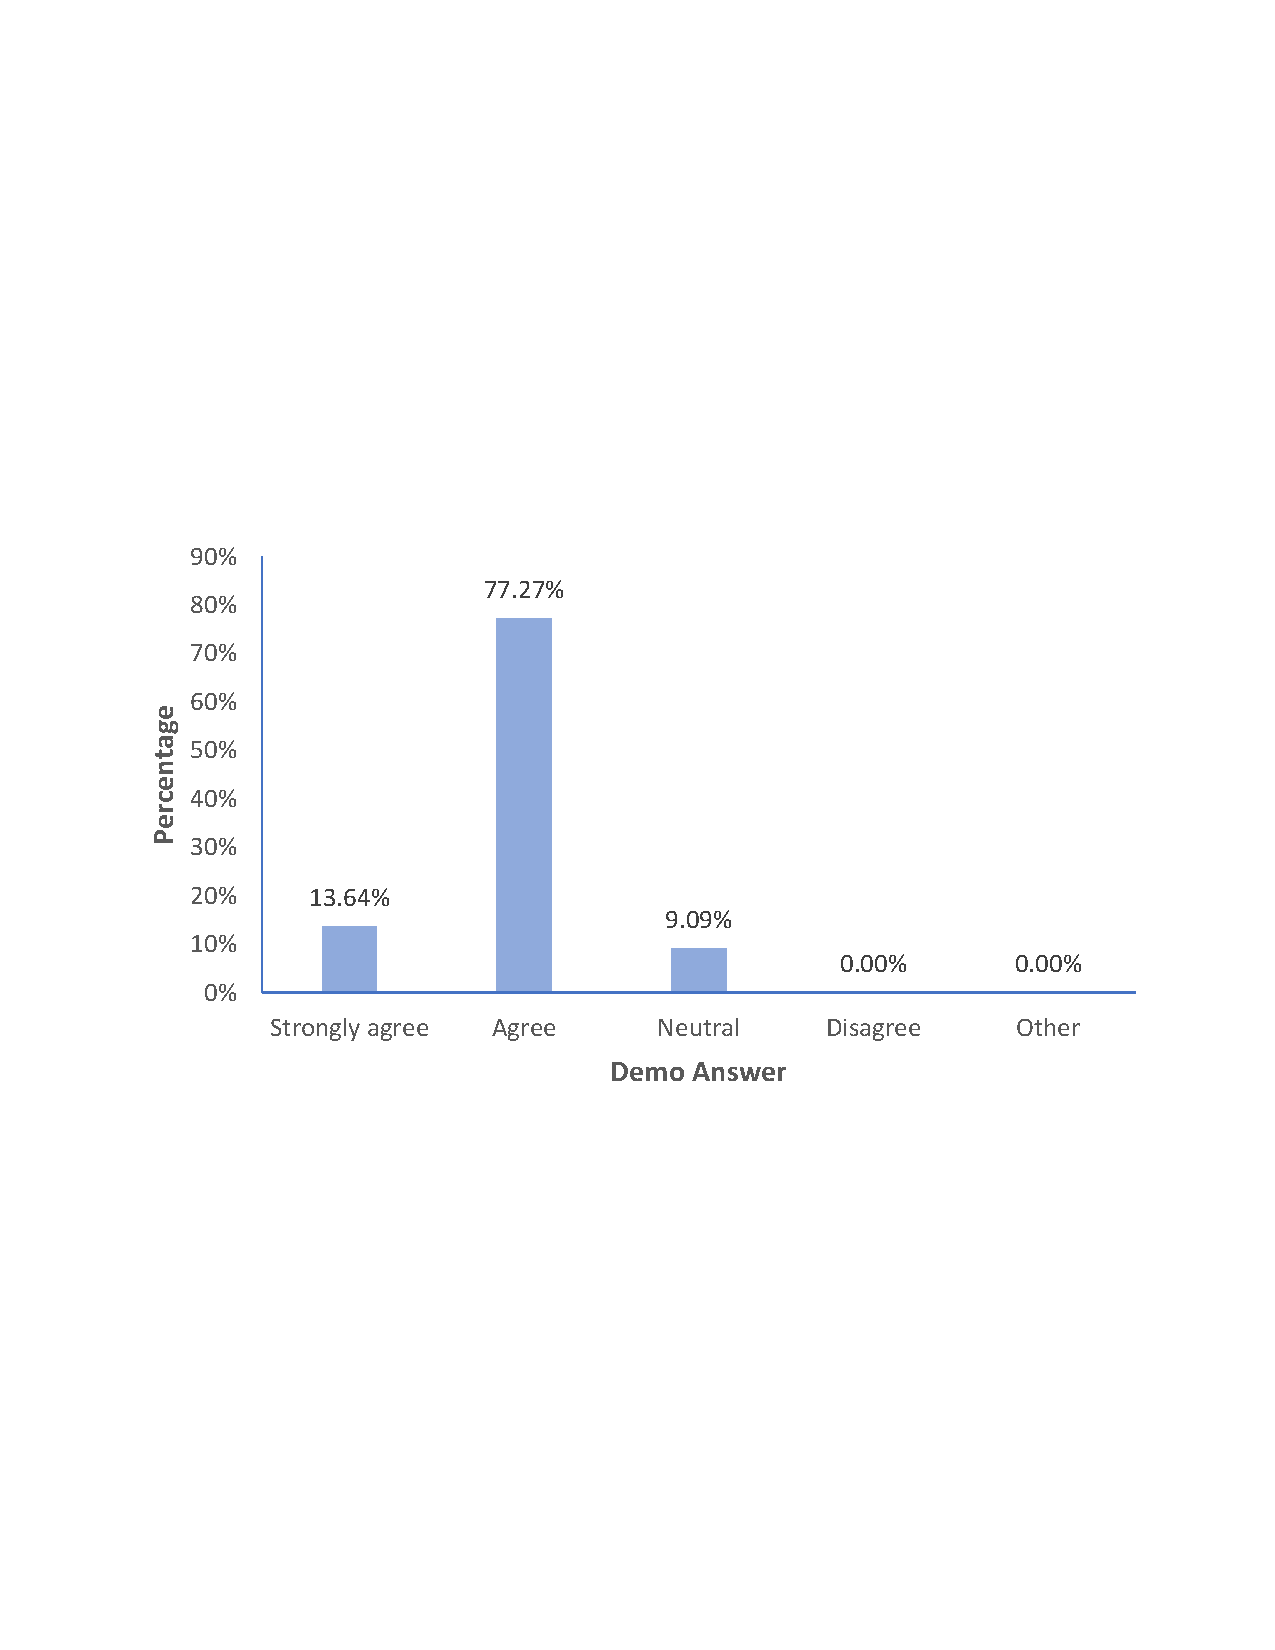
\includegraphics[width=1\textwidth]{study/etu.pdf}
    \caption{The result of online survey - map usability}
    \label{fig:etu}
  \end{center}
\end{figure}

\begin{figure}
  \begin{center}
\subfloat[The evaluation result of map usability by participants\label{fig:etu}]
  {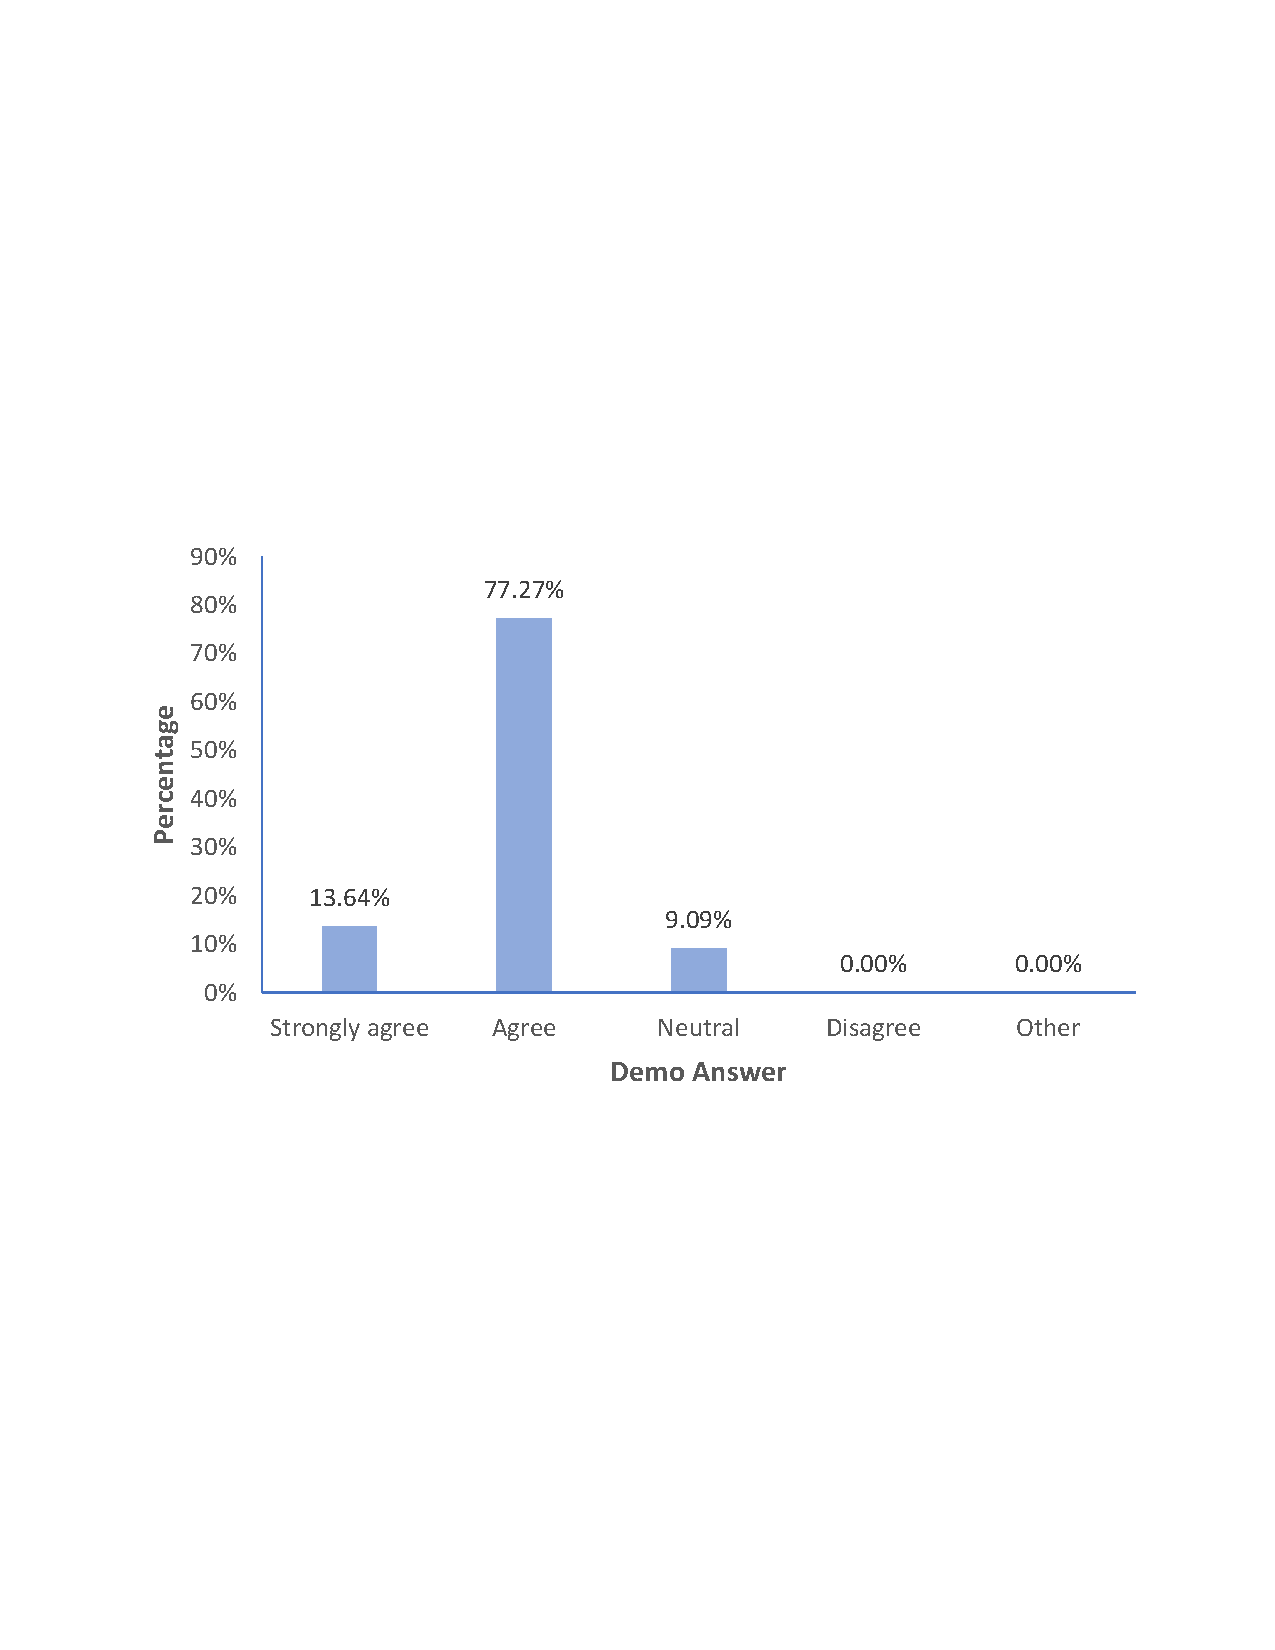
\includegraphics[width=.45\linewidth]{study/etu.pdf}}\hfill
\subfloat[The evaluation result of interface and functionality by participants\label{fig:selfExp}]
  {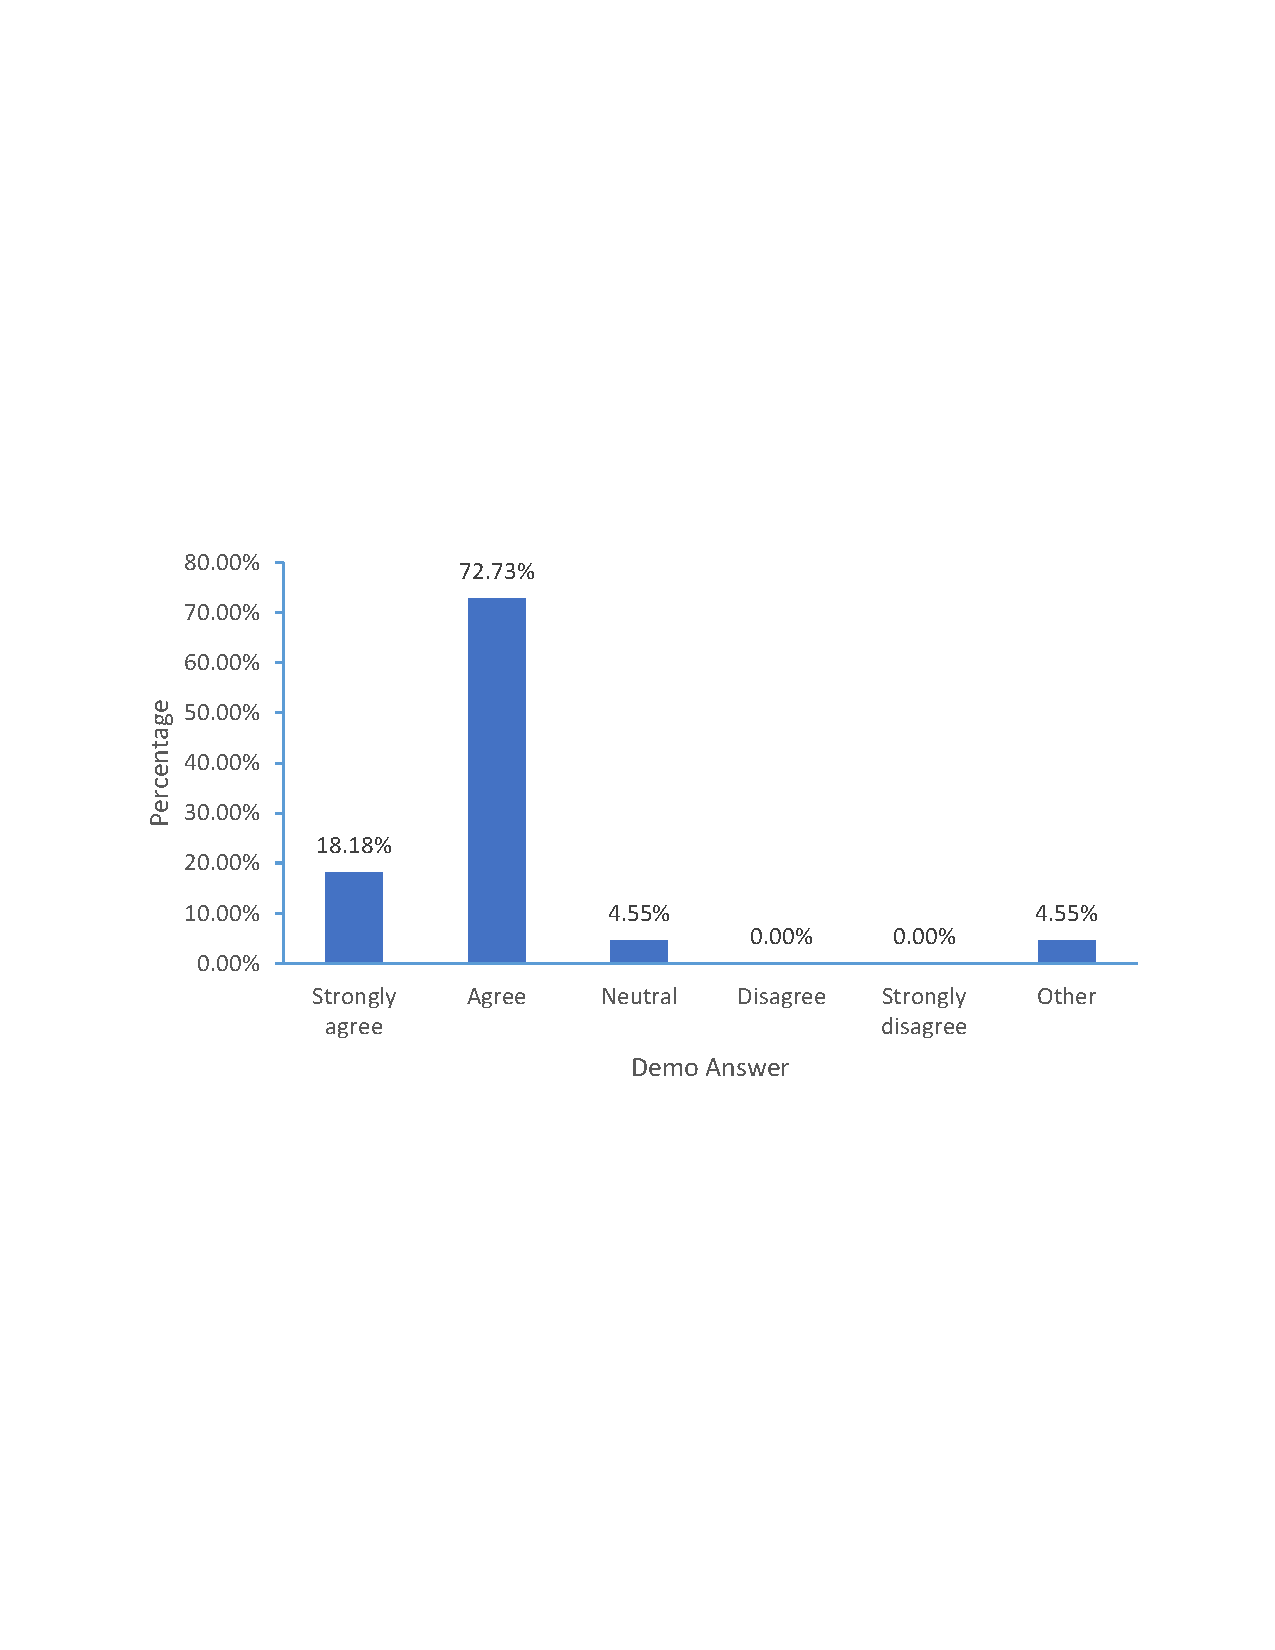
\includegraphics[width=.45\linewidth]{study/selfexp.pdf}}
\hfill
\caption{The evaluation result of online survey}
\label{fig:selfExp}
\end{center}
\end{figure}

\subsection{Working with the Interactive Map}

In this section, the evaluation result of map usability test as well as qualitative comments from the participants are discussed. Each participant of the survey are named with "P" including their id as a suffix (for example participant number 23 is called with "P23"). 

\subsection*{Evaluation of User Interface(UI)}

We assumed that before evaluating the UI, user followed the steps described in the short introduction and gone through the interface accordingly. The purpose of this questionnaire was to evaluate the map UI and its complexity, comprehensibility, interface as well as visual aesthetics. The participants were very positive after using the map and its interface. They found it intuitive and easy to use which is confirmed by the around 91\% participants. Where 77.27\% participants were agreed and around 13.64\% were strongly agreed on the question \textit{“I found the map easy to use”} of the survey (see Figure \ref{fig:etu}). Similar results are also noticed where participants were asked about the structure of map especially the navigation menus, markers, marker pop-ups, buttons, and comparison table. This is confirmed by 91\% (about 72.73\% agreed and 18.18\% strongly agreed) participants on the question \textit{"Interface and functions of this map are self-explanatory"} (see Figure \ref{fig:selfExp}). There was also a comment section where participants can write about their confusions instead of answering the question. P12 said, \textit{"Definitely they are self-explanatory.”} and \textit{"navigation menu could have a logo next to each label”}. 

\subsection*{Evaluation of Map API}

Participants were also asked to evaluate the elements and functions that map API offers. The participants rated the initial cluster view by the average score of 3.81 (standard deviation = 1.40, lowest(strongly disagree) – 1.0, highest – 5.0(strongly agree). This score falls between neutral and agree. A mixed response from the participants on the cluster view is noticed from the high standard deviation. Some of them found it interesting but at the same time, some found it confusing and unnecessary. P12 again commented, \textit{“The power plant density function should be removed, it is only confusing”}. P13 noted the cluster view appears on higher zoom level and said, \textit{“The power plant density representation is not always helping, its appearance can be resolved at higher zoom level”}. The participants found the size of the marker \textit{“Just right”} although some participants found it little bigger, they were satisfied with the icons used inside the marker. The question \textit{“Icons used for power plants are self-explanatory”} got an average score of 4.13 (SD =0.71). Participants also rated the readability of the marker pop-up by the average value of 3.9 (standard deviation = 0.9) and clarity of the navigation menu by the average value of 4.3 (standard deviation = 0.67). Participants found the power line visualization interesting and rated by the average value of 4.5 (standard deviation = 0.60) but not highly satisfied with the loading time in the mobile devices. P2 tested the tool on the mobile device and commented, \textit{“The application crashes very often on tablets while loading power lines”}. This result was expected as we did not use any database for storing large GeoJSON files of power lines. Therefore, it takes between 3 to 5 seconds to load on the map. All in all, the participants found the user interface and other elements of the interface very user friendly and easy to understand.

\subsection*{Evaluation of Comparison table}

The participants also rated the comparison table on the question \textit{“I found the comparison table useful”}. Some participants did not find it useful and it was difficult to find the comparison list.  P2 said, \textit{“Where is the comparison table?”}. One of the reasons for having this difficultly could be a short usage time or they overlooked the short introduction at the beginning. On the other hand, P19 noticed the feature and said, \textit{“Pity that you can compare only the same energy sources”}. All together participants rated this feature by the average score of 3.77 (standard deviation = 1).

\subsection*{Usability Evaluation}

The purpose of this question group was to evaluate the interactive functions, its usability, and usefulness. This study would tell whether the interactive techniques and functions inside the tool suited well for exploring data. From this individual test records, we observed that 75\% of the participants found this map very informative and agreed on the question \textit{“I found this map very informative”}. Others selected neutral as an answer to this question. P9, P11, P2 and P22 mentioned about not having the solar power plant information. P2 was mostly interested in the high voltage transmission line visualization and requested to have more information regarding the transmission lines. P9 said, \textit{“It would be more informative marker pop-up shows the name of the location”}. Around 40\% participants disagreed when they answered the question \textit{“I found the interactivity very complex”} (see Figure \ref{fig:complex}). 30\% participants found it difficult to use because of having less experience in using interactive maps and others decision were neutral. Participants were also asked about the necessity of having a short tutorial beforehand or example of how to use the map. In this case, 55\% participants disagreed just like before and around 15\% were neutral or couldn't decide. Around 15\% participant agree on the question of \textit{“I think that I would need a tutorial before using this visualization tool"} (see Figure \ref{fig:introTutorial}). 

\begin{figure}
  \begin{center}
\subfloat[The evaluation result of - "I found the interactivity very complex"\label{fig:complex}]
  {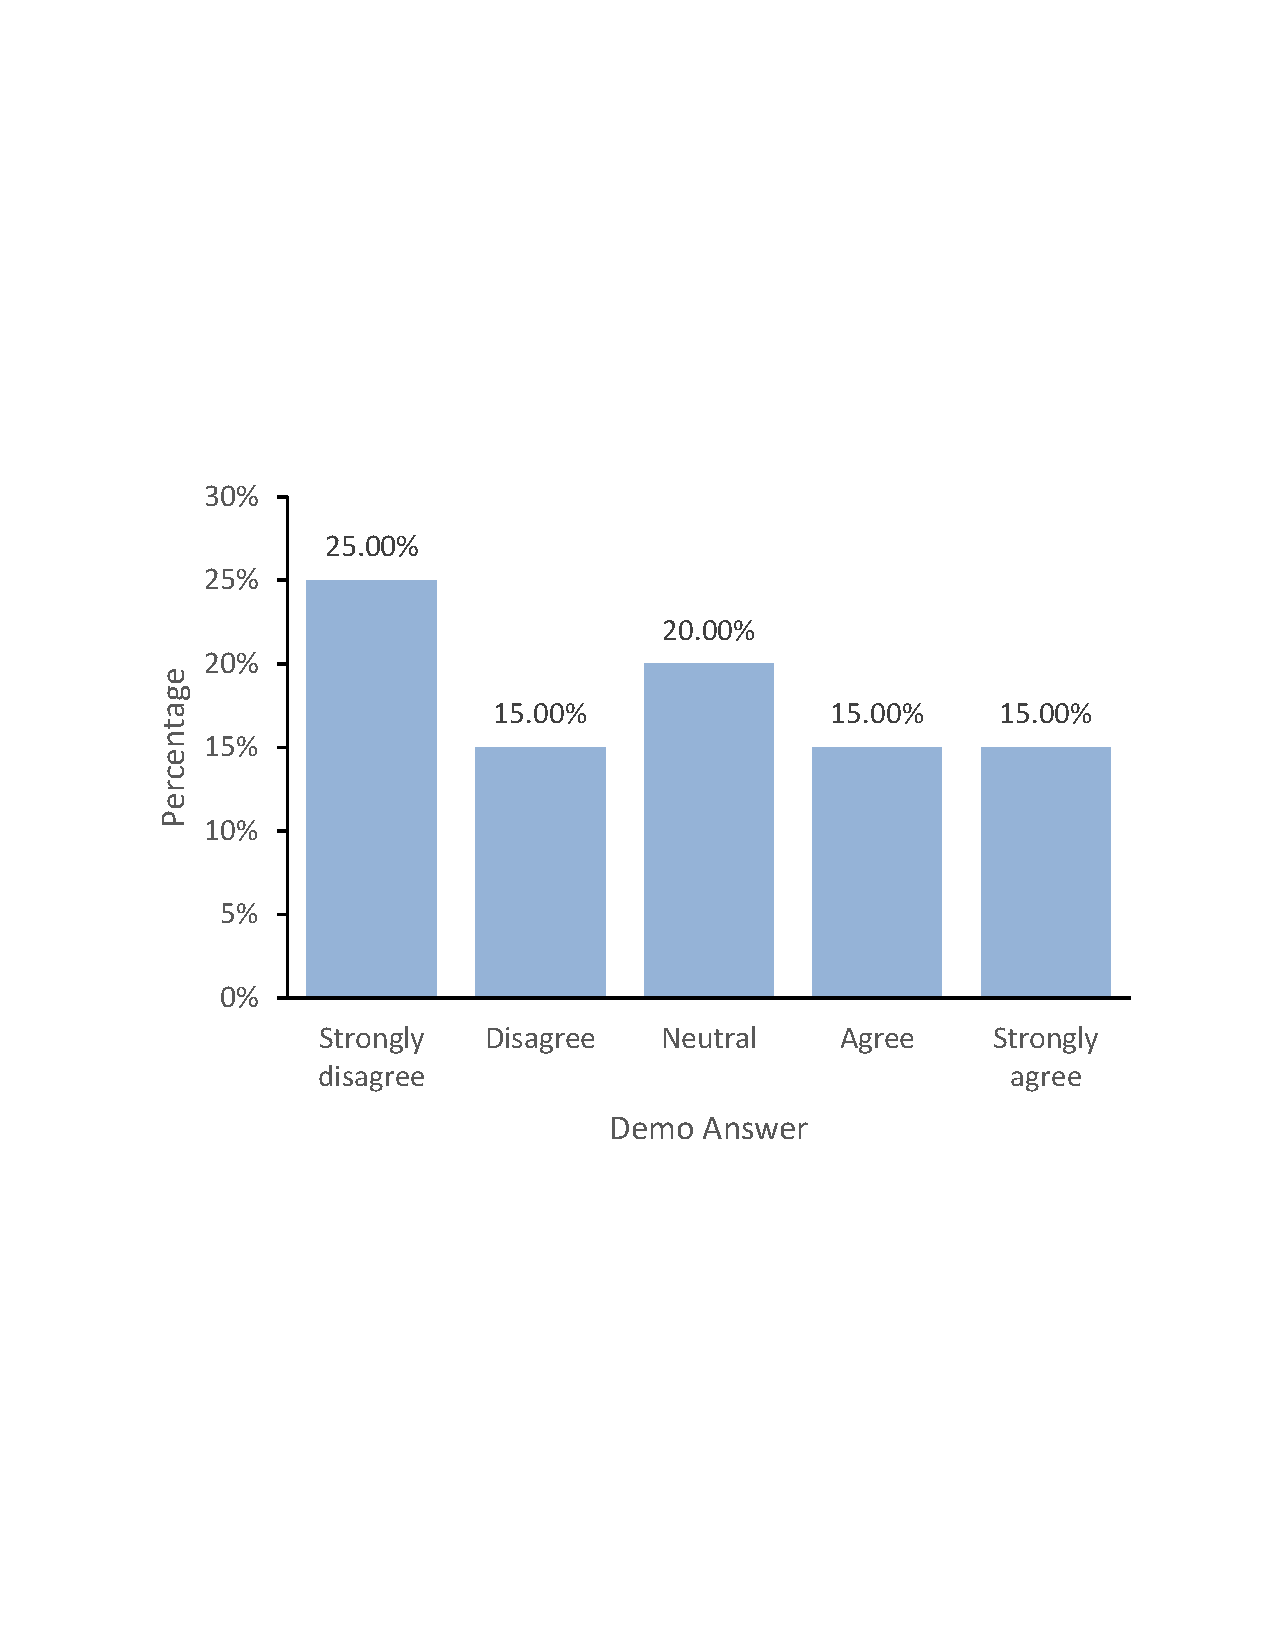
\includegraphics[width=.45\linewidth]{study/complex.pdf}}\hfill
\subfloat[The evaluation result of - "I think that I would need a tutorial before using this visualization tool"\label{fig:introTutorial}]
  {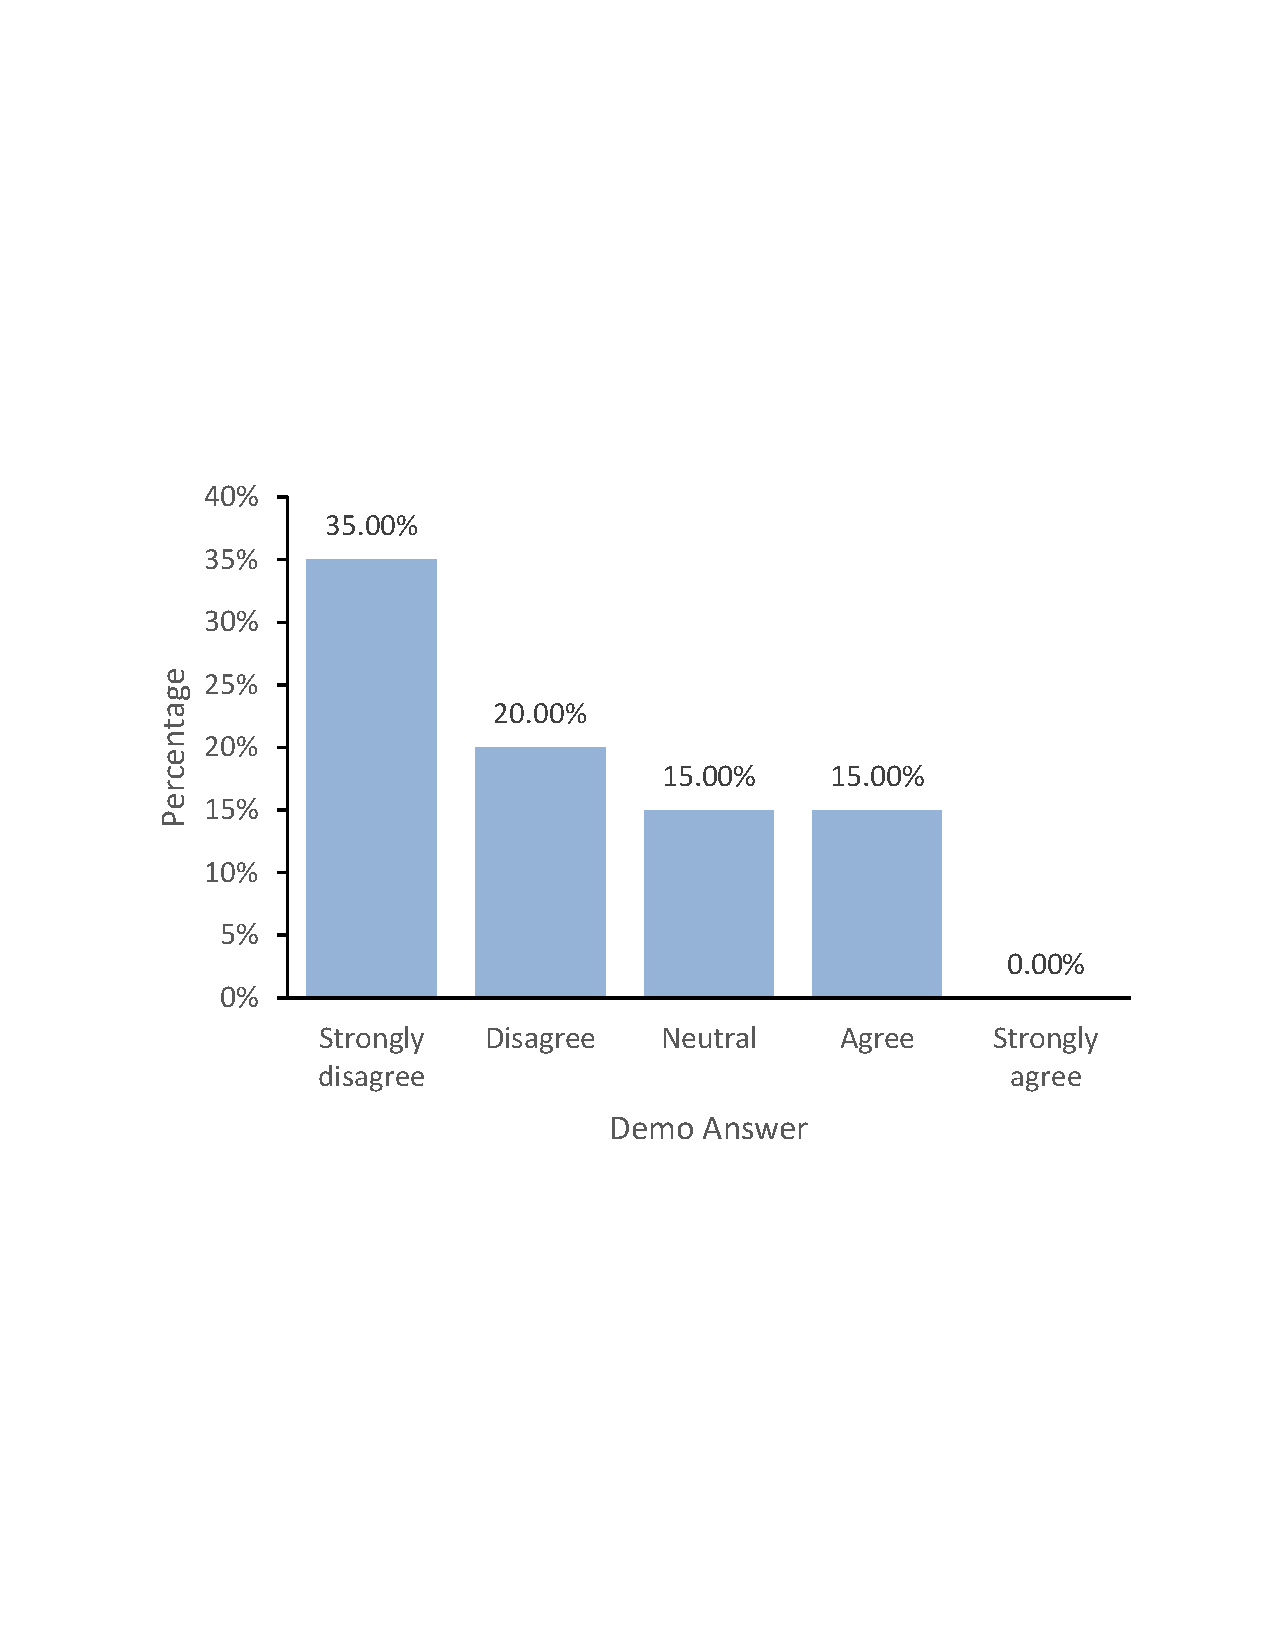
\includegraphics[width=.45\linewidth]{study/intro.pdf}}
\hfill
\caption{The evaluation result of complete visualization tool}
\label{fig:selfExp}
\end{center}
\end{figure}

In figure \ref{fig:finalRev}, the evaluation results are shown ordered by participants based on the map usability and its usefulness. 22 participants completed this question group. Total usability test got a score of 73\%. Where 60\% of the participants rated above than average score and they think the map is very informative and its interactivity is not really complex and around 40\% of the participants found it difficult to use and rated less than the average score.

\begin{figure} 
  \begin{center}
    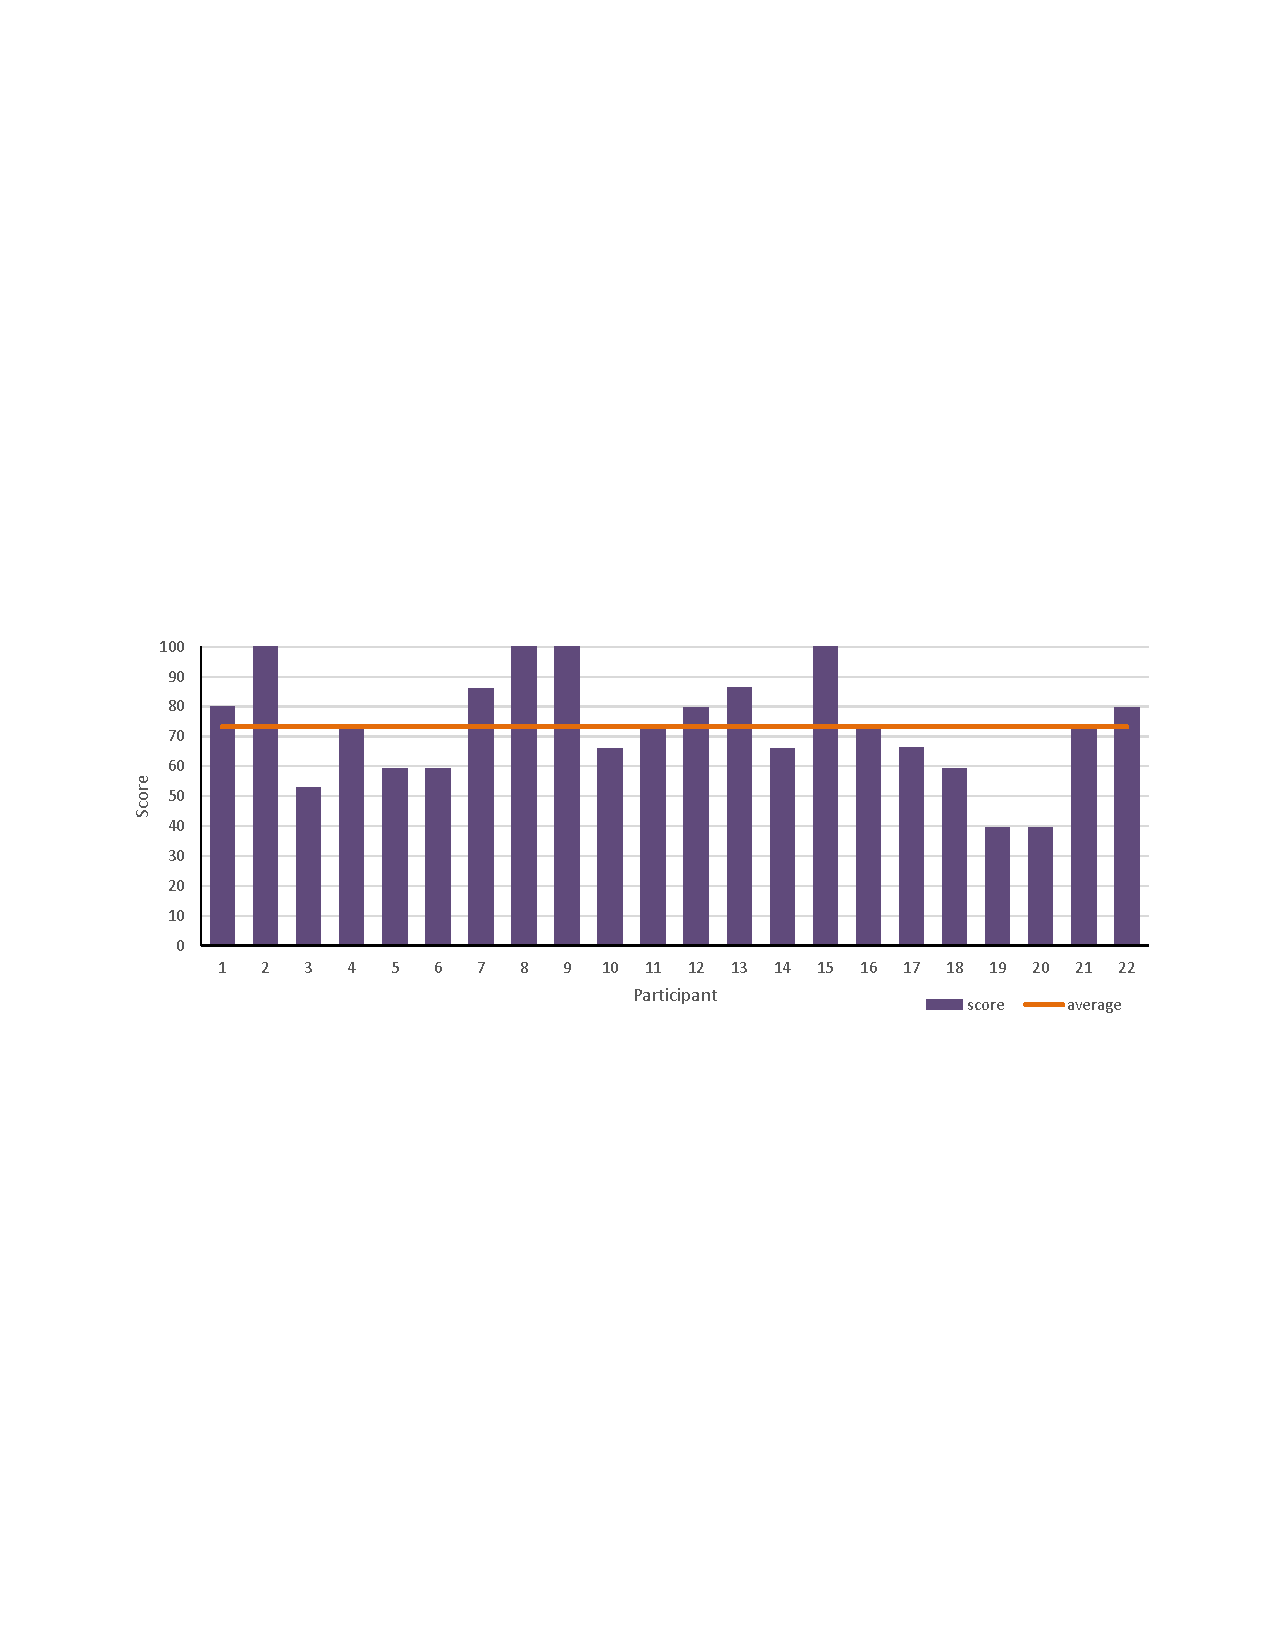
\includegraphics[width=1\textwidth]{study/finalreview.pdf}
    \caption{The result of online survey - complete map usability and usefulness}
    \label{fig:finalRev}
  \end{center}
\end{figure}

\section{User Feedback}

Besides having this information about the power plants the participants in general desired more information from the system. Because of missing information on solar power plants, they proposed to include solar in the information list. Participants also requested to include the city where the plant is located in the marker pop-up. Participants got confused when they saw the marker cluster layer and proposed to omit this feature. The participants also mentioned about difficulties for finding some features, for example, comparison table. Participants also talked about the limitation of comparison table and energy charts. They are interested to compare power plant units from different energy sources on energy chats. They are also interested to see power plants production in bar charts. Participants also requested to have this map in German language. People from social media also shared their thoughts and ideas who didn't participate in the survey. Their thoughts were quite similar with the survey participants. One user said, \textit{“No information on solar!”}. Another social media use provided some important information regarding the correctness of geographical location of power plants.   Another user commented on the 220kV and 380kV power lines and their information. Information provided for the power lines in the map are outdated. However, users from social media noticed the work, got fascinated by the tool and appreciated saying, \textit{“Great Stuff”, "The Map is very informative"}.  

\section{Summary}

The online interactive map was evaluated using an online survey for one week. In this very short time we received 23 survey reports . The study was focused on the qualitative feedback of the map user who are renewable energy professionals, professors, students, engineering working in the energy industry, journalist, and teacher. We were able to reach them through this survey and obtained various feedback, thoughts, ideas, suggestion, usability evaluation result as well as appreciations. The qualitative feedback however uncovered some gaps and limitations within the tool which can be included in the list of future work.
